\subsubsection{Guiding Diffusion with Lightweight Autoregressive Model}


% The beauty of diffusion model is the ability of producing tokens without relying on the iterative decoding process, whereas the inc
To address this token incoherence challenge~(Challenge \circled{2}) from Section~\ref{sec:incor}
and fully exploit the parallelism of diffusion process, we propose \texttt{Guided Diffusion}. 
% \begin{figure}[t!]
\vspace{-6pt}
\begin{figure}[H]
    \centering
    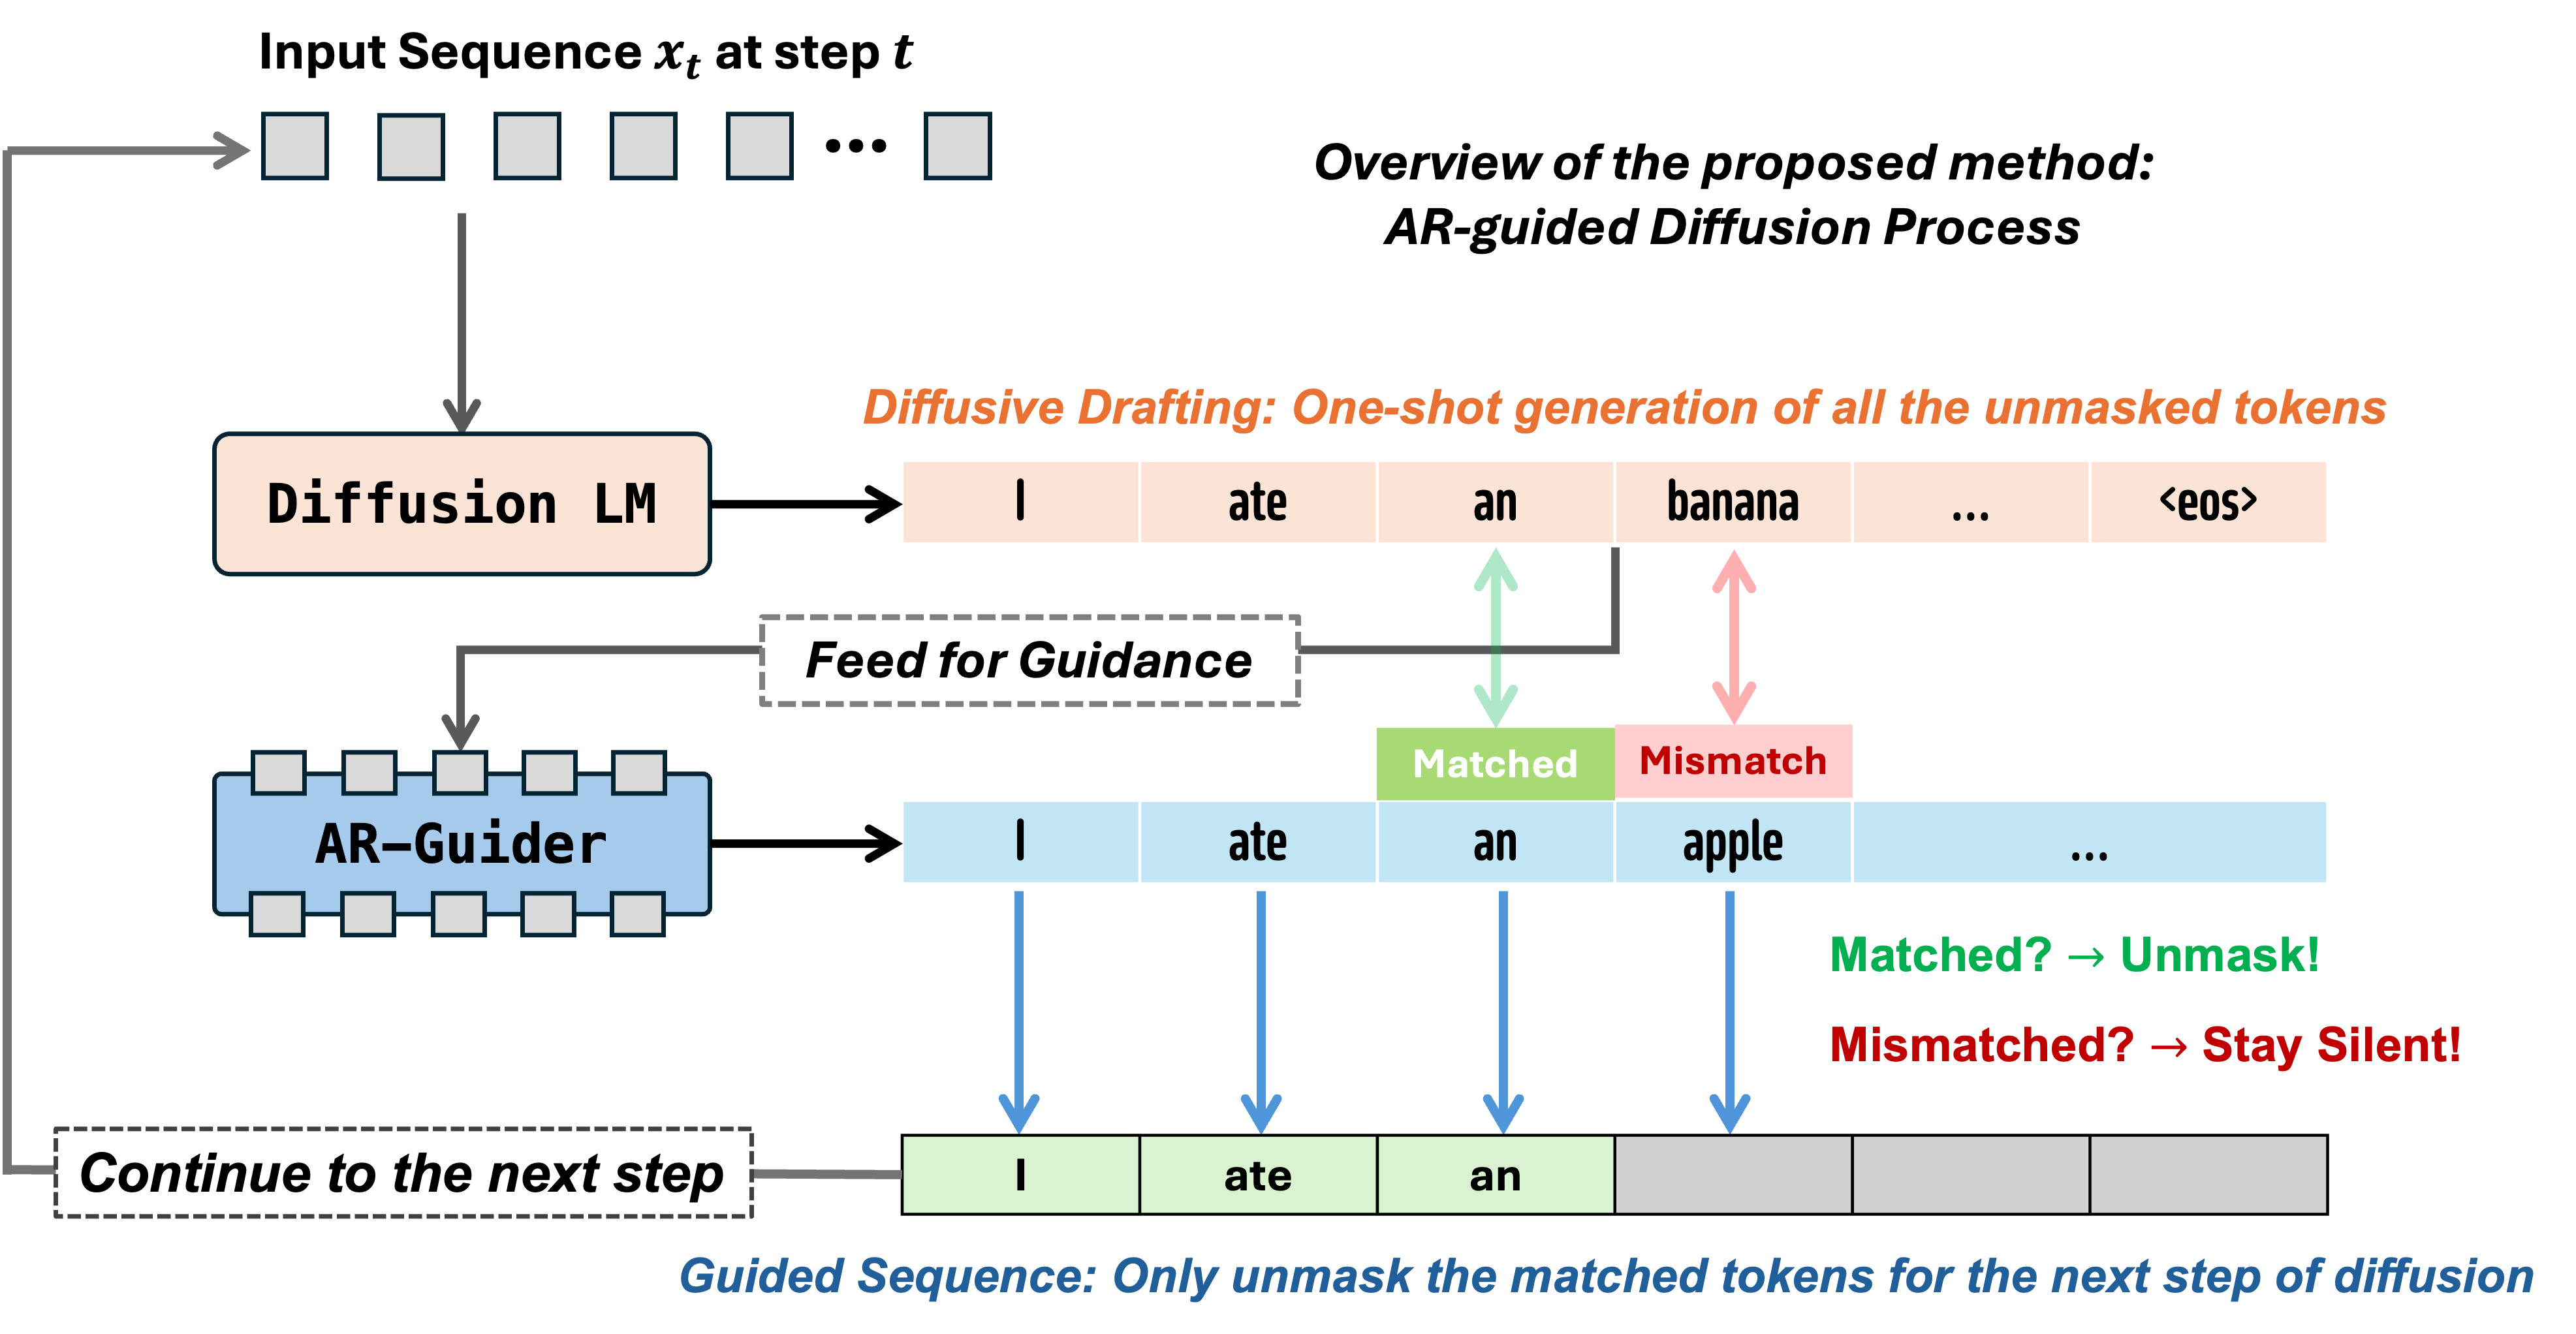
\includegraphics[width=\linewidth]{sections/method/figures/guided_diffusion.png}
    \caption{AR-guided Diffusion Model. The diffusion model performs a one-step diffusion process, followed by a one-time forward pass of the AR guider. The matched tokens are unmasked for the next step of diffusion.}
    \label{fig:guided_diffusion}
\end{figure}
\vspace{-6pt}

Specifically, we leverage the diffusion model as the ``drafter'' model by first unmasking \textbf{all} the tokens with one step. 
The masked tokens predicted by the diffusion model are only unmasked when they are consistent with the predictions from the autoregressive LM model, as shown in Figure~\ref{fig:guided_diffusion}. 
For the scenario when the matching ratio between the diffusion drafter and auto-regressive model is zero, the guided diffusion will only accept the one free tokens from the AR model output. 

This cross-model agreement serves as a lightweight coherence prior, enabling the model to safely unmask multiple tokens in parallel, without requiring any additional training or fine-tuning.

% In contrast to prior heuristic-based methods (e.g., confidence thresholds or top-$k$ logits), which often suffer from severe quality degradation when unmasking more than a few tokens per step, guided diffusion maintains fluency and correctness even under aggressive unmasking. This substantially reduces the number of denoising steps, often by a factor of 5× or more, without compromising output quality.

% We provide detailed comparisons in Section~\ref{sec:experiments}, \zhanqiu{TODO} showing that guided diffusion achieves significantly faster inference and stronger generation quality compared to baseline sampling strategies.


Guided diffusion performs iterative unmasking by coordinating predictions from a diffusion language model (DLM) and a frozen autoregressive model (ARM). At each denoising step, instead of relying on heuristic confidence thresholds, it uses agreement between the two models to decide how many tokens to safely unmask.

Formally, let \( x_T \in \mathbb{N}^L \) be the current sequence containing masked and unmasked tokens. The diffusion model \( f_\theta \) predicts logits over vocabulary tokens at all masked positions, from which we take the Top-1 predictions:
\[
t^{\text{DLM}} = \text{argmax}( \operatorname{Softmax}(f_\theta(x))).
\]
These proposed tokens are fed to the ARM \( g_\phi \), which produces a second set of logits:
\[
t^{\text{ARM}} = \text{argmax}( \operatorname{Softmax}(g_\phi(t^{\text{DLM}}))).
\]
Let \( M = [i_1, \dots, i_m] \subseteq \{1, \dots, L\} \) denote the current masked positions in \(x\). We compute the largest prefix length \(k\) such that
\[
t^{\text{DLM}}_{i_j} = t^{\text{ARM}}_{i_j} \quad \text{for all } j \le k.
\]
If \(k > 0\), we unmask positions \(i_1, \dots, i_k\) using the DLM proposals. If no agreement is found, we conservatively unmask only the first token \(i_1\). This process is repeated until all tokens are unmasked.

This decoding strategy allows the model to adaptively control the amount of parallel unmasking based on model confidence and alignment, enabling efficient generation without compromising output quality.
We present the details of the proposed method in Algorithm~\ref{alg:guided_diffusion}.

We would like to highlight that the proposed \texttt{Guided Diffusion} properly combines the advantages of \textbf{both} diffusion model and auto-regressive model. 
For each guiding step, \textbf{both} one-time diffusion process from the drafter and the one-time forward pass of the auto-regressive model are fast, while the guidance from the auto-regressive model facilitates the coherence of the diffused output tokens with improved semantical logic. 

\textbf{Guided Diffusion vs. Speculative Decoding.} 
Unlike speculative decoding, \texttt{Guided Diffusion} does not require token-wise correction from the auto-regressive model. In other words, the proposed method produces output sequence \textbf{without} introducing the repetitive correction process, which guarantees the latency benefits obtained from the fast diffusion process. 
Speculative decoding uses a small AR model for autoregressive drafting, followed by the big model correction. On the contrary, the proposed guided diffusion flips the paradigm by maximizing the drafting efficiency of the big diffusion model. To that end, the reasoning power of the diffusion model is fully preserved, while the AR guider model simply ensures the causality of the output. 


% In the meantime, Guided Diffusion can be smoothly transformed into ``Guided Correction''. The correction step can be directly applied after selecting the optimal tokens for unmasking. 
% In particular, when a stronger or domain-specific auto-regressive model is available, we can optionally apply a correction step that overwrites the diffusion draft with the accurate output from the expert auto-regressive model, as presented in Algorithm~\ref{alg:guided_diffusion_corrected}. We presented the detailed results 

%The original algorithm relies entirely on the diffusion model’s generation, but when a stronger or domain-specific ARM is available, we can optionally apply a correction step that overwrites the diffusion model’s proposal using the ARM’s prediction to improve accuracy, as shown in Algorithm~\ref{alg:guided_diffusion_corrected}.


